\section{Evaluación de Alternativas}
\label{alternatives}

\subsection{Técnicas de Downsampling}

Una vez introducido el concepto de downsampling como solución al problema de visualización de series de tiempo muy densas, es necesario revisar y comparar las principales alternativas existentes.

Diversos autores han propuesto algoritmos que permiten seleccionar los puntos más representativos de una serie para facilitar su visualización. A continuación, se presenta un resumen de los métodos más relevantes:

\begin{enumerate}
    \item \textbf{Mode-Median-Bucket (MMB)}: 
    Divide los datos en bloques y selecciona un punto por bloque usando la moda o la mediana de los valores. Es simple y fácil de entender, pero tiende a omitir picos y valles locales relevantes~\cite{steinarsson2013downsampling}.

    \item \textbf{Min-Std-Error-Bucket (MSEB)}: 
    Utiliza regresión lineal para calcular el error estándar entre pares de puntos, eligiendo aquellos que minimizan la suma de errores. Produce resultados estadísticamente coherentes, pero suaviza demasiado la serie y elimina detalles visuales importantes~\cite{steinarsson2013downsampling}.

    \item \textbf{Longest-Line-Bucket (LLB)}: 
    Similar a MSEB, pero en lugar de minimizar el error, maximiza la longitud total de las líneas entre puntos seleccionados. Tiene mejor capacidad para conservar picos extremos y fluctuaciones relevantes~\cite{steinarsson2013downsampling}.

    \item \textbf{Largest-Triangle-Three-Buckets (LTTB)}: 
    Divide los datos en tres bloques consecutivos y selecciona el punto que forma el triángulo de mayor área con los puntos de los bloques adyacentes. Esta técnica preserva bien la forma general del gráfico y es eficiente computacionalmente~\cite{steinarsson2013downsampling}.

    \item \textbf{Largest-Triangle-Dynamic (LTD)}: 
    Variante del LTTB que adapta dinámicamente el tamaño de los bloques según la variación local de los datos. Mejora la representación visual en series con regiones muy fluctuantes y otras más estables~\cite{steinarsson2013downsampling}.

    \item \textbf{MinMaxLTTB}: 
    Propuesto por Van Der Donckt {\it et al.}~\cite{vanderdonckt2023minmaxlttb}, este algoritmo mejora la escalabilidad de LTTB al aplicar una preselección eficiente de puntos mínimos y máximos verticales mediante el algoritmo MinMax, para luego aplicar LTTB solo sobre esos puntos seleccionados. De esta manera, reduce significativamente el tiempo de cómputo sin sacrificar calidad visual.
\end{enumerate}

Dado el enfoque de este trabajo, se seleccionó principalmente el uso del algoritmo \textbf{MinMaxLTTB}. Esta decisión se fundamenta en varios factores: en primer lugar, el algoritmo ha sido propuesto por los mismos autores que desarrollaron la biblioteca \texttt{tsdownsample}, lo que garantiza una implementación de referencia optimizada y bien documentada. Además, MinMaxLTTB presenta un excelente equilibrio entre rendimiento y fidelidad visual, al combinar una reducción sustancial en el tiempo de cómputo con una buena preservación de la forma general de la serie de tiempo.

Como complemento para el análisis comparativo, también se utilizará el algoritmo \textbf{LTTB}, ya que es ampliamente citado en la literatura como una opción base eficiente, y su comparación directa con MinMaxLTTB permite observar el impacto de la estrategia de preselección aplicada por los autores.

\subsection{Estructuras de Datos Compactas}

El uso de estructuras de datos compactas permite representar secuencias numéricas en memoria utilizando una menor cantidad de bits por elemento, manteniendo el acceso a los datos sin pérdida de información. 

En la literatura existen bibliotecas que implementan estas estructuras de datos compactas. En particular, utilizaremos la biblioteca \texttt{sdsl4py}, un conjunto de bindings en Python para la Succinct Data Structure Library (SDSL), que permite acceder a múltiples representaciones compactas desde  Python. A continuación se presentan las  estructuras de datos compactas que fueron consideradas en esta memoria de título:

\begin{enumerate}
    \item \texttt{enc\_vector\_elias\_gamma}: 
        Utiliza codificación de enteros Elias-Gamma. Es eficiente para valores pequeños, ya que su tamaño codificado crece logarítmicamente con el valor. No puede representar ceros.
        
        \begin{enumerate}
            \item Para cada entero \(x_i > 0\):
            \begin{enumerate}
                \item Se convierte a binario: \(\text{bin}(x_i)\)
                \item Se calcula su longitud en bits: \(\mathcal{L} = \lfloor \log_2 x_i \rfloor + 1\)
                \item Se anteponen \(\mathcal{L} - 1\) ceros al binario
                \item El código resultante es: \texttt{prefijo + binario}
            \end{enumerate}
            \item Para decodificar:
            \begin{enumerate}
                \item Contar ceros iniciales (\(z\)) → \(\mathcal{L} = z + 1\)
                \item Leer los siguientes \(\mathcal{L}\) bits
                \item Interpretar ese bloque como un entero
                \item Repetir hasta terminar el bitstream
            \end{enumerate}
        \end{enumerate}
    
        \begin{figure}
            \centering
            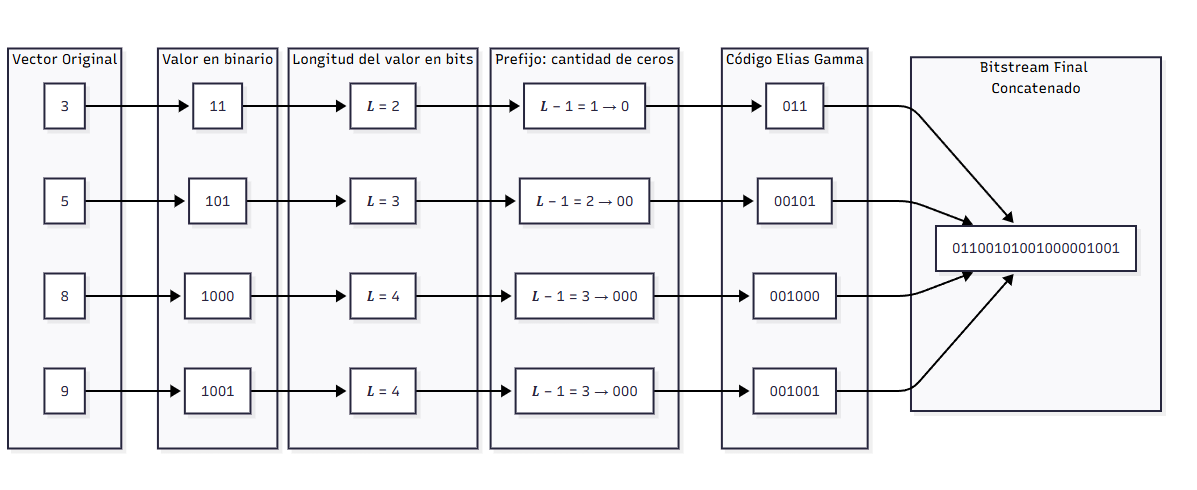
\includegraphics[width=0.9\linewidth]{alternatives/images/enc_vector_elias_gamma.png}
            \caption[Ejemplo \texttt{enc\_vector\_elias_gamma}]{Diagrama paso a paso de codificación usando el tipo de vector \texttt{enc\_vector} y la codificación \textit{Elias Gamma}.}
            \label{enc_vector_elias_gamma}
        \end{figure}
    
    \item \texttt{enc\_vector\_elias\_delta}: 
        Variante de Elias-Gamma que mejora la compresión para valores grandes, manteniendo eficiencia en lectura. También requiere que todos los valores sean mayores que cero.
            
        \begin{enumerate}
            \item Para cada entero \(x_i > 0\):
            \begin{enumerate}
                \item Se calcula su longitud en bits: \(\mathcal{L} = \lfloor \log_2 x_i \rfloor + 1\)
                \item Se codifica \(\mathcal{L}\) usando Elias Gamma
                \item Se eliminan el bit más significativo de \(\text{bin}(x_i)\) y se concatenan al código anterior
                \item El código resultante es: \(\text{EliasGamma}(\mathcal{L}) + \text{bin}(x_i)[2:]\)
            \end{enumerate}
            \item Para decodificar:
            \begin{enumerate}
                \item Decodificar un número \( \mathcal{L} \) usando Elias Gamma
                \item Leer los siguientes \(\mathcal{L} - 1\) bits
                \item Anteponer un bit 1 a esa secuencia
                \item Interpretar el binario resultante como un entero
            \end{enumerate}
        \end{enumerate}
        
        \begin{figure}
            \centering
            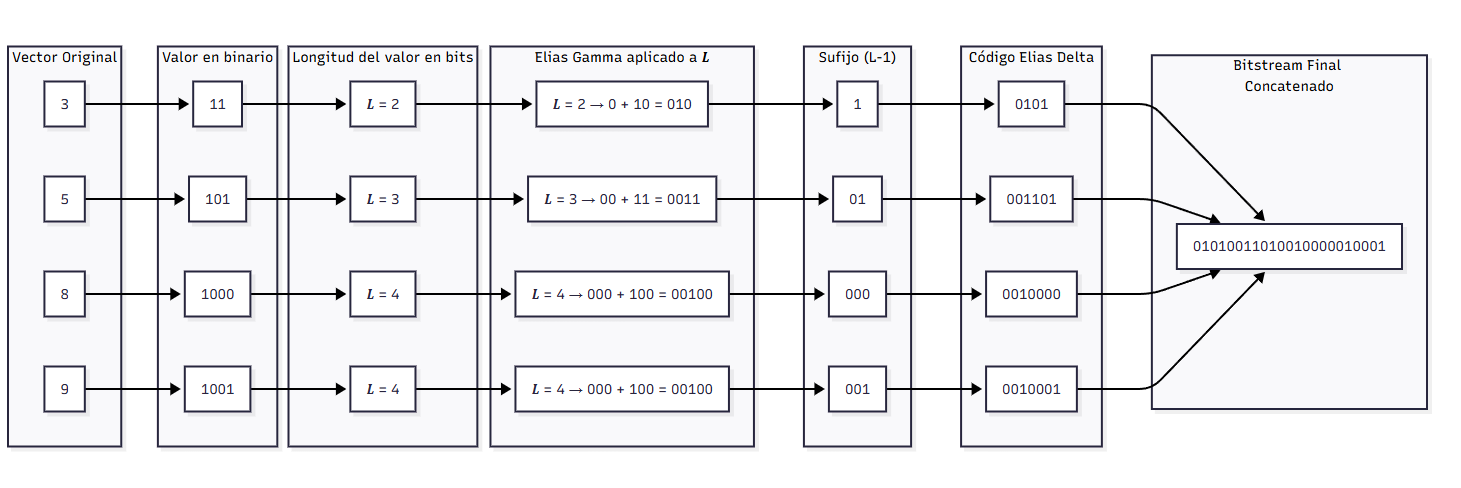
\includegraphics[width=0.9\linewidth]{alternatives/images/enc_vector_elias_delta.png}
            \caption[Ejemplo \texttt{enc\_vector\_elias\_delta}]{Diagrama paso a paso de codificación usando el tipo de vector \texttt{enc\_vector} y la codificación \textit{Elias Delta}.}
            \label{enc_vector_elias_delta}
        \end{figure}
        

    \item \texttt{enc\_vector\_fibonacci}:
        Usa codificación basada en la sucesión de Fibonacci. Esta técnica es compacta y libre de prefijos, pero tiene limitaciones para valores cero y una complejidad levemente mayor en decodificación.
        
        \begin{enumerate}
            \item Para cada entero \(x_i > 0\):
            \begin{enumerate}
                \item Se representa como suma de términos no consecutivos de la sucesión de Fibonacci (codificación de Zeckendorf).
                \item Se escribe un bit por cada número de Fibonacci menor o igual a \(x_i\): se marca con un 1 si se usa y con 0 si no.
                \item Se agrega un bit 1 al final como terminador.
            \end{enumerate}
        
            \item Para decodificar:
            \begin{enumerate}
                \item Leer bits hasta encontrar dos 1 seguidos (el 1 de terminación).
                \item Interpretar los 1s como los términos de Fibonacci usados.
                \item Sumar los términos correspondientes para obtener el valor original.
            \end{enumerate}
        \end{enumerate}
        
        \begin{figure}
            \centering
            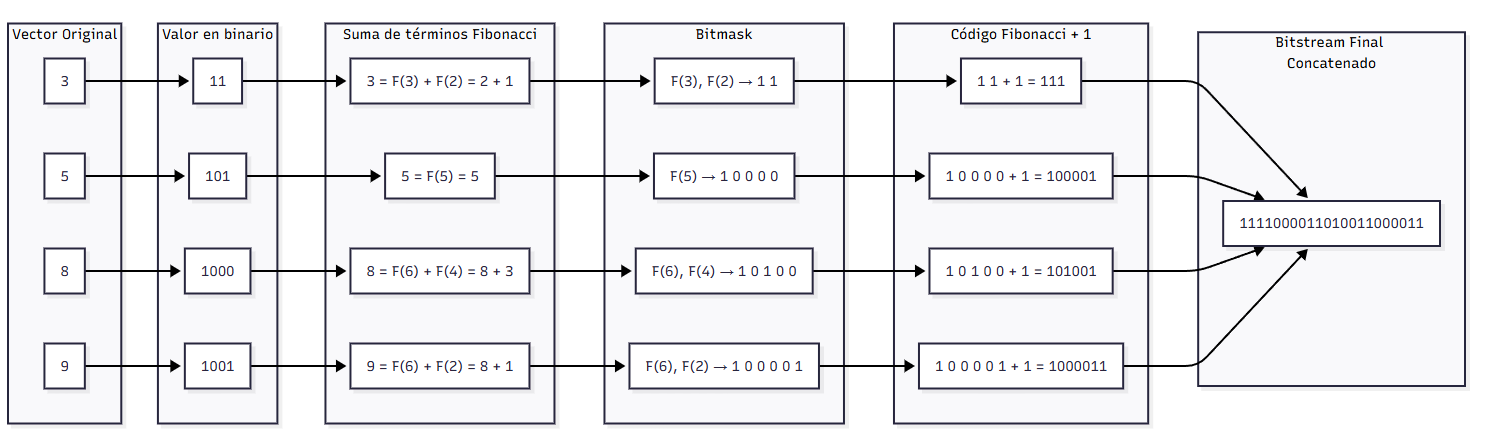
\includegraphics[width=0.9\linewidth]{alternatives/images/enc_vector_fibonacci.png}
            \caption[Ejemplo \texttt{enc\_vector\_fibonacci}]{Diagrama paso a paso de codificación usando el tipo de vector \texttt{enc\_vector} y la codificación \textit{Fibonacci}.}
            \label{enc_vector_fibonacci}
        \end{figure}
        

  \item \texttt{enc\_vector\_comma\_2}:  
        Codificación por comas binarias usando una base derivada de un ancho fijo de dígitos (\(t_{\text{width}} = 2\)). Es simple y compacta para valores enteros positivos, ideal para secuencias con pocos valores grandes.
        
        \begin{enumerate}
            \item Para cada entero \(x_i > 0\):
            \begin{enumerate}
                \item Se define una base \(b = 2^{t_{\text{width}}} - 1 = 3\)
                \item Se representa el número en base \(b\): \(\text{base}_b(x_i)\)
                \item Cada dígito de esa representación se codifica en binario con \(t_{\text{width}}\) bits
                \item Se agrega un dígito de terminación con valor \(b\) (es decir, el número reservado para marcar el final), también con \(t_{\text{width}}\) bits
            \end{enumerate}
            \item Para decodificar:
            \begin{enumerate}
                \item Se leen bloques de \(t_{\text{width}}\) bits
                \item Cada bloque se interpreta como un dígito en base \(b\)
                \item Cuando se detecta un bloque igual a \(b\), se termina la lectura del número
                \item Se reconstruye el entero a partir de la secuencia de dígitos previa al terminador
            \end{enumerate}
        \end{enumerate}
        
        \begin{figure}
            \centering
            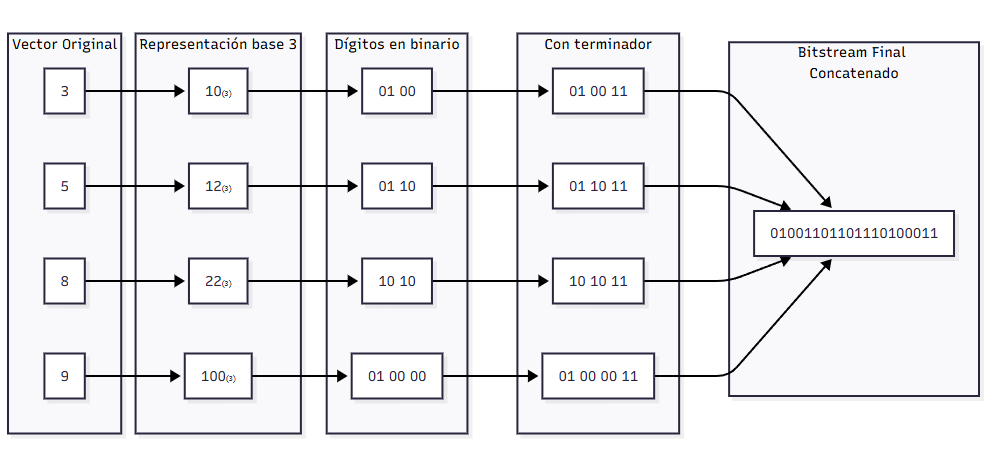
\includegraphics[width=0.9\linewidth]{alternatives/images/enc_vector_comma.png}
            \caption[Ejemplo \texttt{enc\_vector\_comma\_2}]{Diagrama paso a paso de codificación usando el tipo de vector \texttt{enc\_vector} con codificación por comas binarias (base \(2^2 - 1 = 3\)).}
            \label{enc_vector_comma_2}
        \end{figure}
        
        
  \item \texttt{vlc\_vector\_elias\_delta}:  
        Variante optimizada del tipo \texttt{enc\_vector\_elias\_delta}, que agrega una estructura de muestreo para permitir acceso aleatorio más eficiente. Los elementos se codifican igual que en Elias Delta, pero se almacenan junto con un índice que permite ubicar cada cierto número de elementos directamente en el bitstream.
    
        \begin{enumerate}
            \item Para construir el vector:
            \begin{enumerate}
                \item Se codifica cada valor \(x_i > 0\) como \(x_i + 1\) usando Elias Delta.
                \item El resultado se concatena en un bitstream global \(m_z\).
                \item Cada \(t_{\text{dens}}\) elementos (por ejemplo, cada 2), se registra la posición de bit de inicio como una muestra (sample).
                \item Se guarda un vector con las posiciones de muestra: \texttt{m\_sample\_pointer}.
            \end{enumerate}
    
            \item Para decodificar el elemento \(x_i\):
            \begin{enumerate}
                \item Se calcula el bloque de muestra \(j = \lfloor i / t_{\text{dens}} \rfloor\)
                \item Se toma el bit de inicio \(p = \texttt{m\_sample\_pointer}[j]\)
                \item Se decodifican los siguientes \(i \bmod t_{\text{dens}} + 1\) elementos desde el bitstream, a partir de \(p\)
                \item Finalmente, se le resta 1 al valor decodificado
            \end{enumerate}
        \end{enumerate}
    
        \begin{figure}[h!]
            \centering
            \makebox[\textwidth][c]{%
                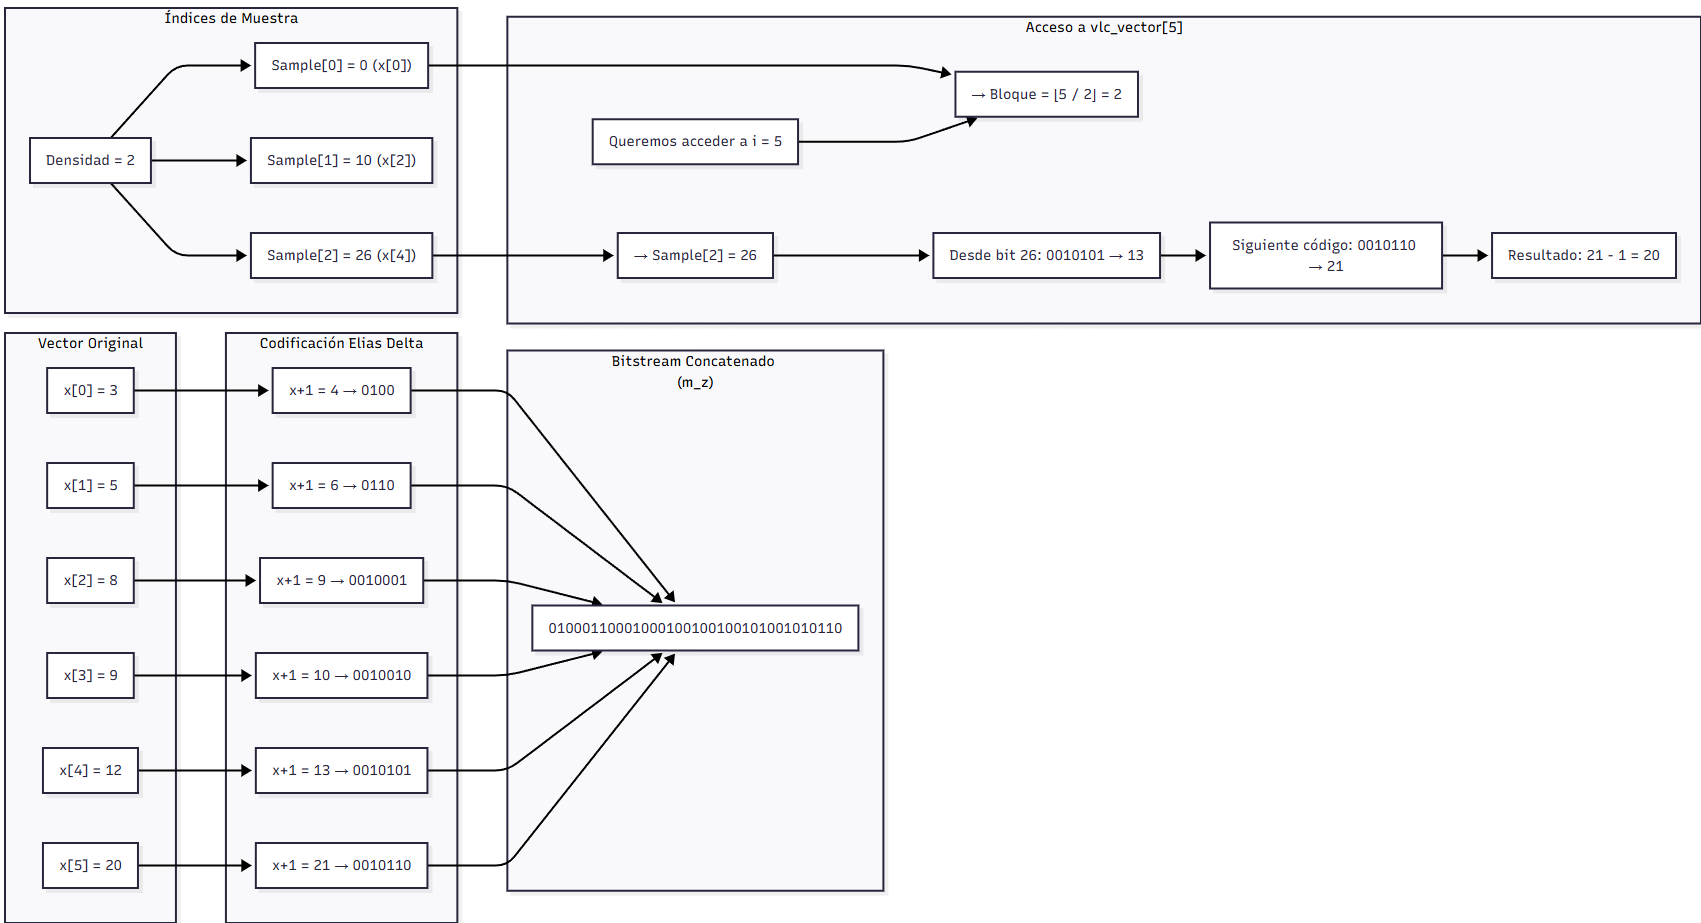
\includegraphics[width=1.1\textwidth]{alternatives/images/vlc_vector_elias_delta.png}
            }
            \caption[Ejemplo \texttt{vlc\_vector\_elias\_delta}]{Acceso eficiente con \texttt{vlc\_vector} codificado con \textit{Elias Delta} y muestreo. Se muestran los pasos de codificación, almacenamiento del bitstream y búsqueda rápida gracias a los índices de muestra.}
            \label{vlc_vector_elias_delta}
        \end{figure}
        
            
    

    \item \textbf{vlc\_vector\_elias\_gamma}:
    Equivalente a la anterior, pero usando codificación Elias-Gamma. Útil cuando se prioriza el acceso sobre la compresión máxima.

    \item \textbf{vlc\_vector\_fibonacci}:
    Combina las ventajas de codificación Fibonacci con accesos más eficientes mediante índices auxiliares.

    \item \textbf{vlc\_vector\_comma\_2}:
    Aplica codificación comma-2 con estructura de acceso rápido. Es útil cuando se necesita acceder a datos comprimidos con latencias bajas.

    \item \texttt{dac\_vector}:
        Utiliza \textit{Directly Addressable Codes} (DAC), una estructura escalonada que permite un buen balance entre compresión y velocidad de acceso. Es especialmente útil para secuencias de enteros donde los valores tienen alta varianza.
        
        \begin{enumerate}
            \item Para codificar un entero \(x_i > 0\):
            \begin{enumerate}
                \item Se representa en binario: \(\text{bin}(x_i)\)
                \item Se divide en bloques de \(t_{\text{width}}\) bits desde el bit más significativo.
                \item Cada bloque se guarda en un nivel diferente de la estructura DAC.
                \item Se usa un bit de continuación por cada bloque (excepto el último) para señalar si hay más bloques en niveles inferiores.
            \end{enumerate}
    
            \item Para decodificar:
            \begin{enumerate}
                \item Se comienza en el primer nivel, leyendo un bloque de \(t_{\text{width}}\) bits y su bit de continuación.
                \item Si el bit indica continuación, se avanza al siguiente nivel y se repite el proceso.
                \item Se concatenan los bloques hasta que el bit de continuación sea 0.
                \item El binario resultante es el valor original.
            \end{enumerate}
        \end{enumerate}
        
        \begin{figure}
            \centering
            \makebox[\textwidth][c]{%
                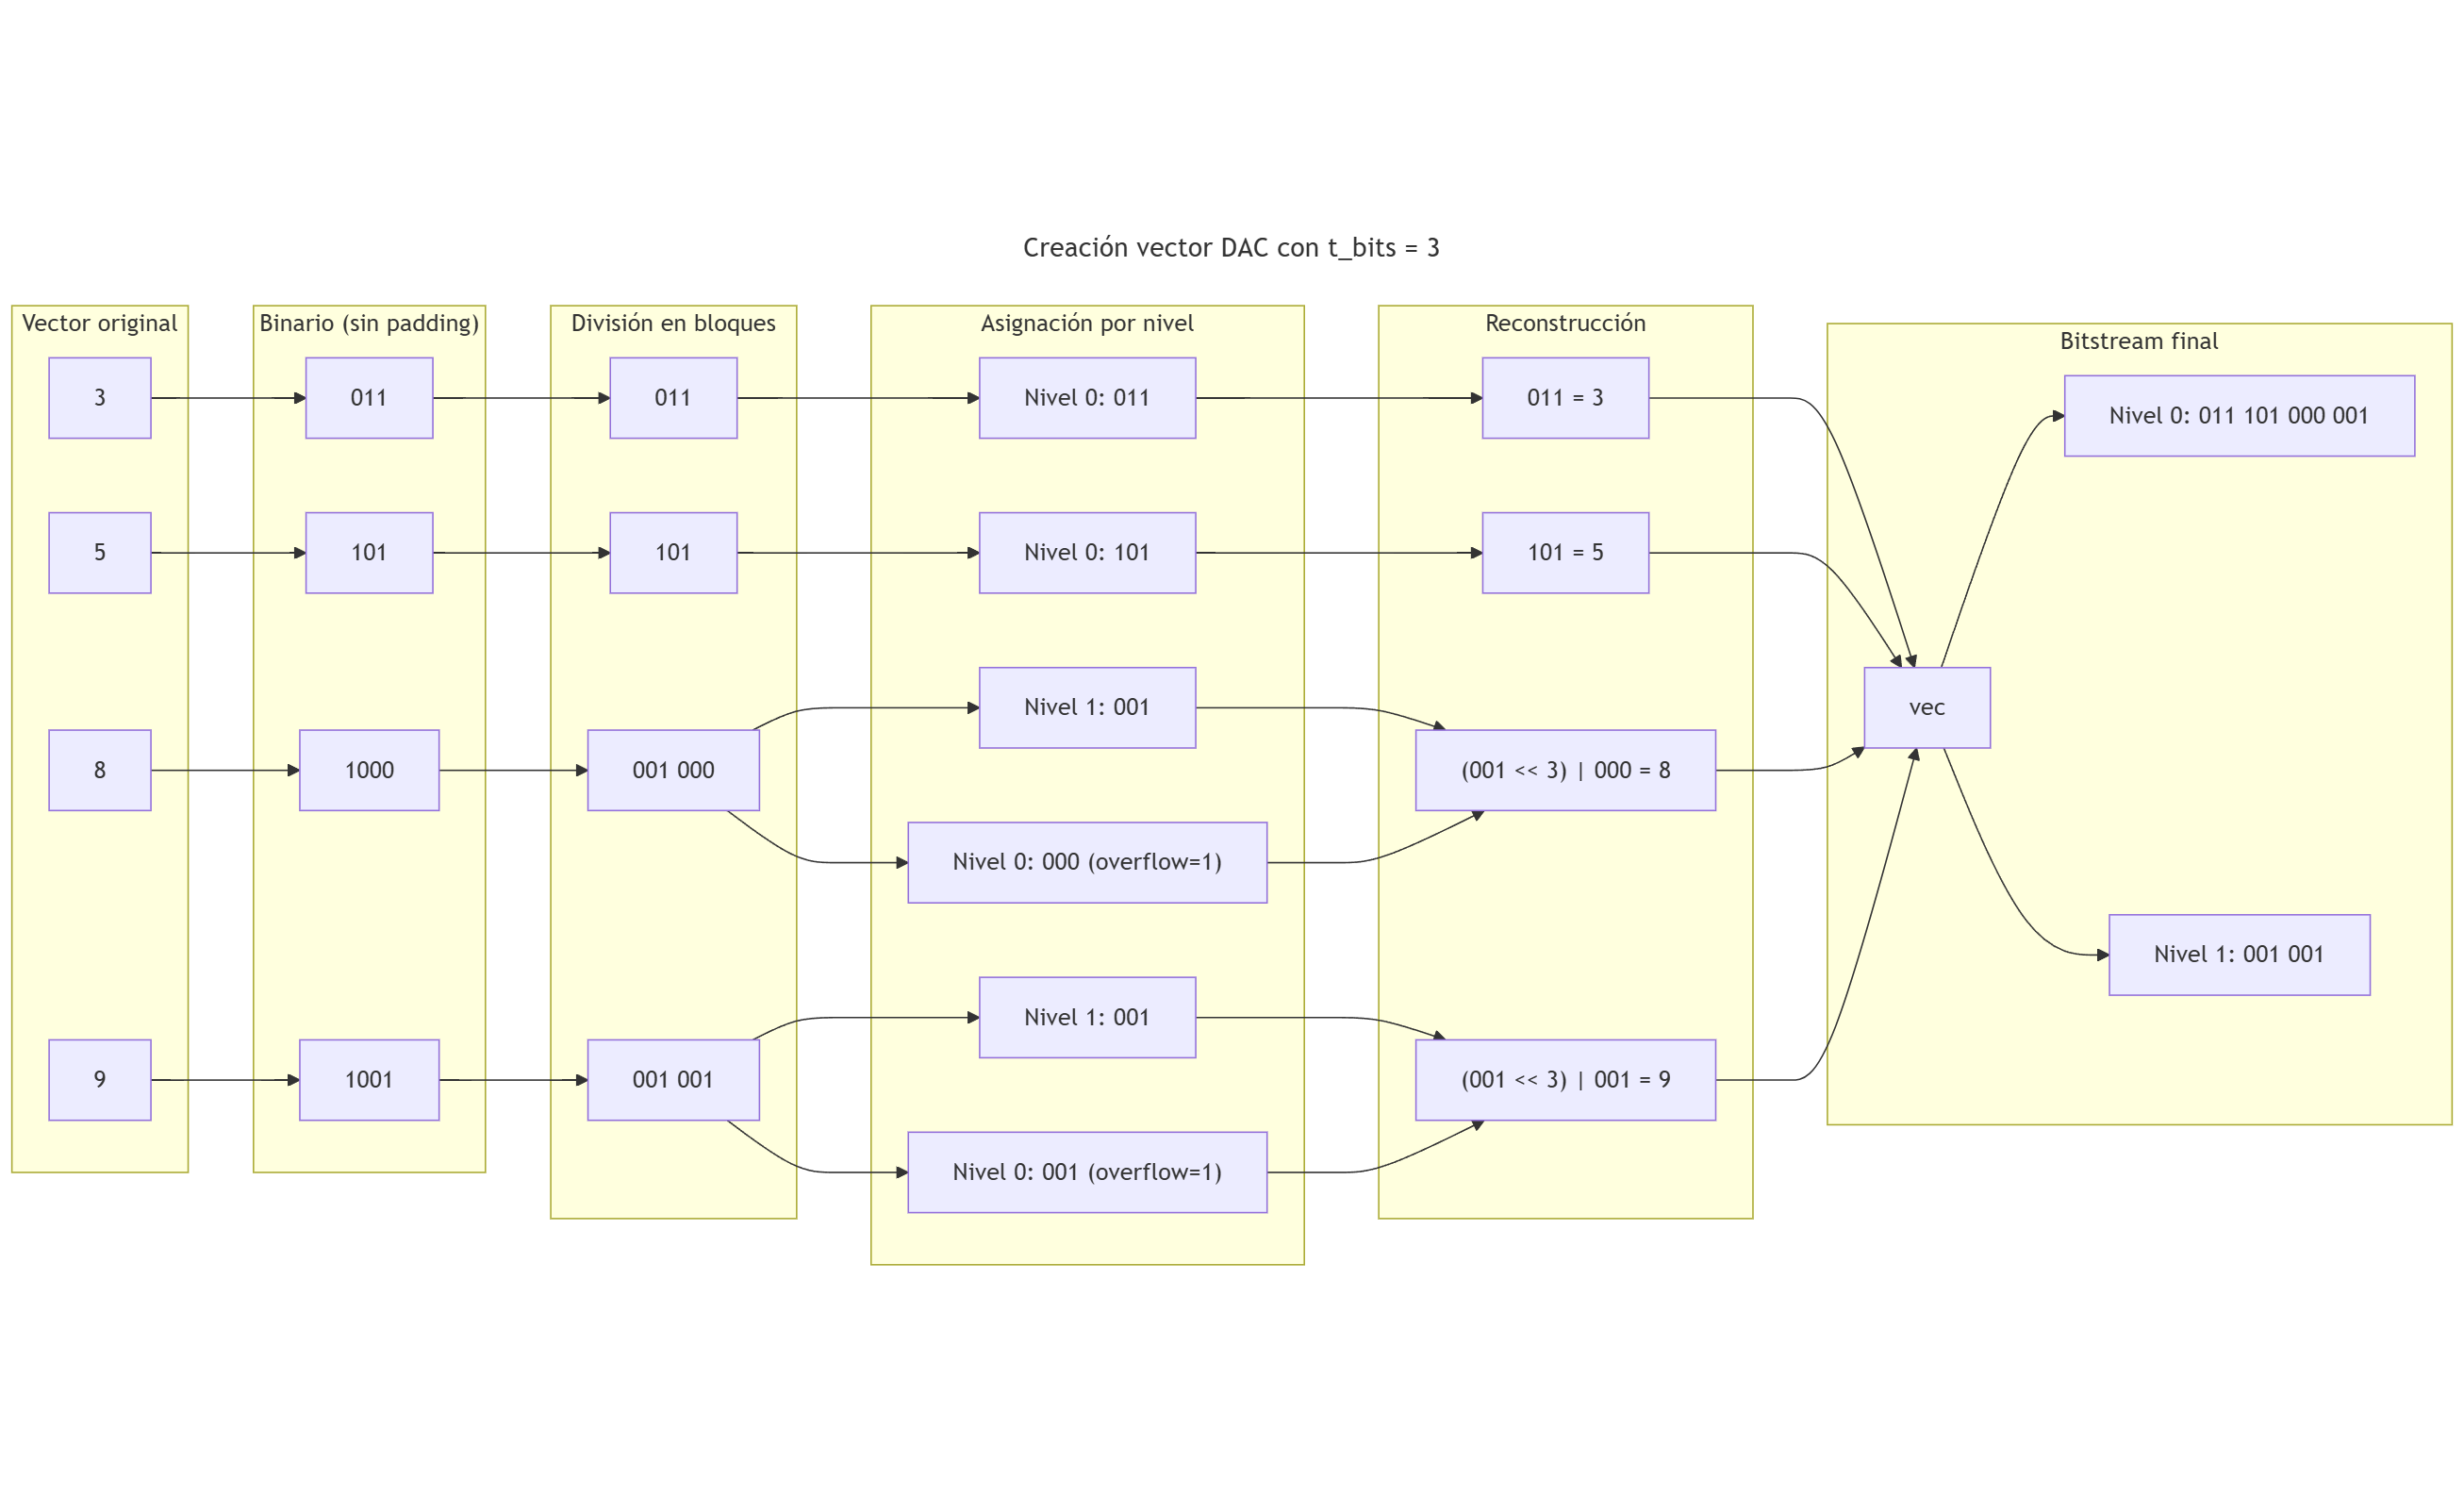
\includegraphics[width=1.3\textwidth]{alternatives/images/dac_vector.png}
            }
            \caption[Ejemplo \texttt{dac\_vector}]{Estructura escalonada del vector \texttt{dac\_vector}. Cada nivel almacena bloques de bits fijos con su correspondiente bit de continuación, permitiendo acceso eficiente sin necesidad de decodificar secuencialmente todo el vector.}
            \label{dac_vector}
        \end{figure}


\end{enumerate}

Para evaluar estas estructuras de datos, se han medido tres métricas clave: el tiempo de acceso a los elementos, el tiempo de construcción de la estructura y el espacio utilizado en memoria. 

Es importante mencionar que debido a las limitantes de la implementación de \texttt{enc\_vector} dentro de la biblioteca \texttt{sdsl4py}, se ha omitido la estructura para su evaluación y posterior experimentación. 

\paragraph{Input}
\vspace{0.2cm}

Para garantizar una evaluación comprehensiva y representativa del comportamiento de las estructuras de datos comprimidas, se han diseñado cuatro tipos de vectores sintéticos que simulan diferentes patrones de datos comúnmente encontrados en aplicaciones reales:

\begin{enumerate}
    \item \textbf{Incremental pequeño (\texttt{incremental\_small}):} Vectores con valores crecientes que presentan pequeñas diferencias entre elementos consecutivos. Este patrón simula series temporales con crecimiento gradual o datos de sensores con variaciones mínimas. Los valores de $x$ siguen la secuencia $[1, 2, 3, ..., n]$, mientras que los valores de $y$ añaden una pequeña variación aleatoria en el rango $[0, 2]$ a cada posición.

    \item \textbf{Aleatorio (\texttt{random}):} Vectores con valores completamente aleatorios distribuidos uniformemente en un rango amplio. Este patrón representa el peor caso para algoritmos de compresión, ya que no presenta patrones predecibles. Tanto $x$ como $y$ contienen enteros aleatorios en el rango $[1, n \times 10]$.

    \item \textbf{Oscilante (\texttt{oscillating}):} Vectores que siguen un patrón de onda sinusoidal, alternando entre valores ascendentes y descendentes. Este comportamiento es típico en señales periódicas, datos de vibración o patrones cíclicos. Los valores de $x$ son secuenciales, mientras que $y$ sigue la función $y_i = \frac{n}{2}(1 + \sin(\frac{4\pi i}{n}))$.

    \item \textbf{Incremental grande (\texttt{incremental\_large}):} Vectores con valores crecientes que presentan grandes diferencias entre elementos consecutivos. Los valores de $x$ son secuenciales $[1, 2, 3, ..., n]$, y los valores de $y$ se calculan como $y_i = i \times \text{random}[50, 200]$.
\end{enumerate}

Cada vector de prueba contiene por defecto 10,000 elementos, proporcionando un volumen de datos suficiente para evaluar el rendimiento de las estructuras de datos compactas. Esta diversidad de patrones permite analizar cómo cada método de compresión se adapta a diferentes características de los datos, desde el caso ideal (datos con alta correlación) hasta el caso más desafiante (datos completamente aleatorios).

\paragraph{Resultados}
A continuación, se presenta un promedio de los resultados obtenidos al evaluar las distintas estructuras de datos compactas utilizando los vectores sintéticos mencionados anteriormente.

% añadir imagenes y tablas de resultados
\begin{figure}[H]
\centering
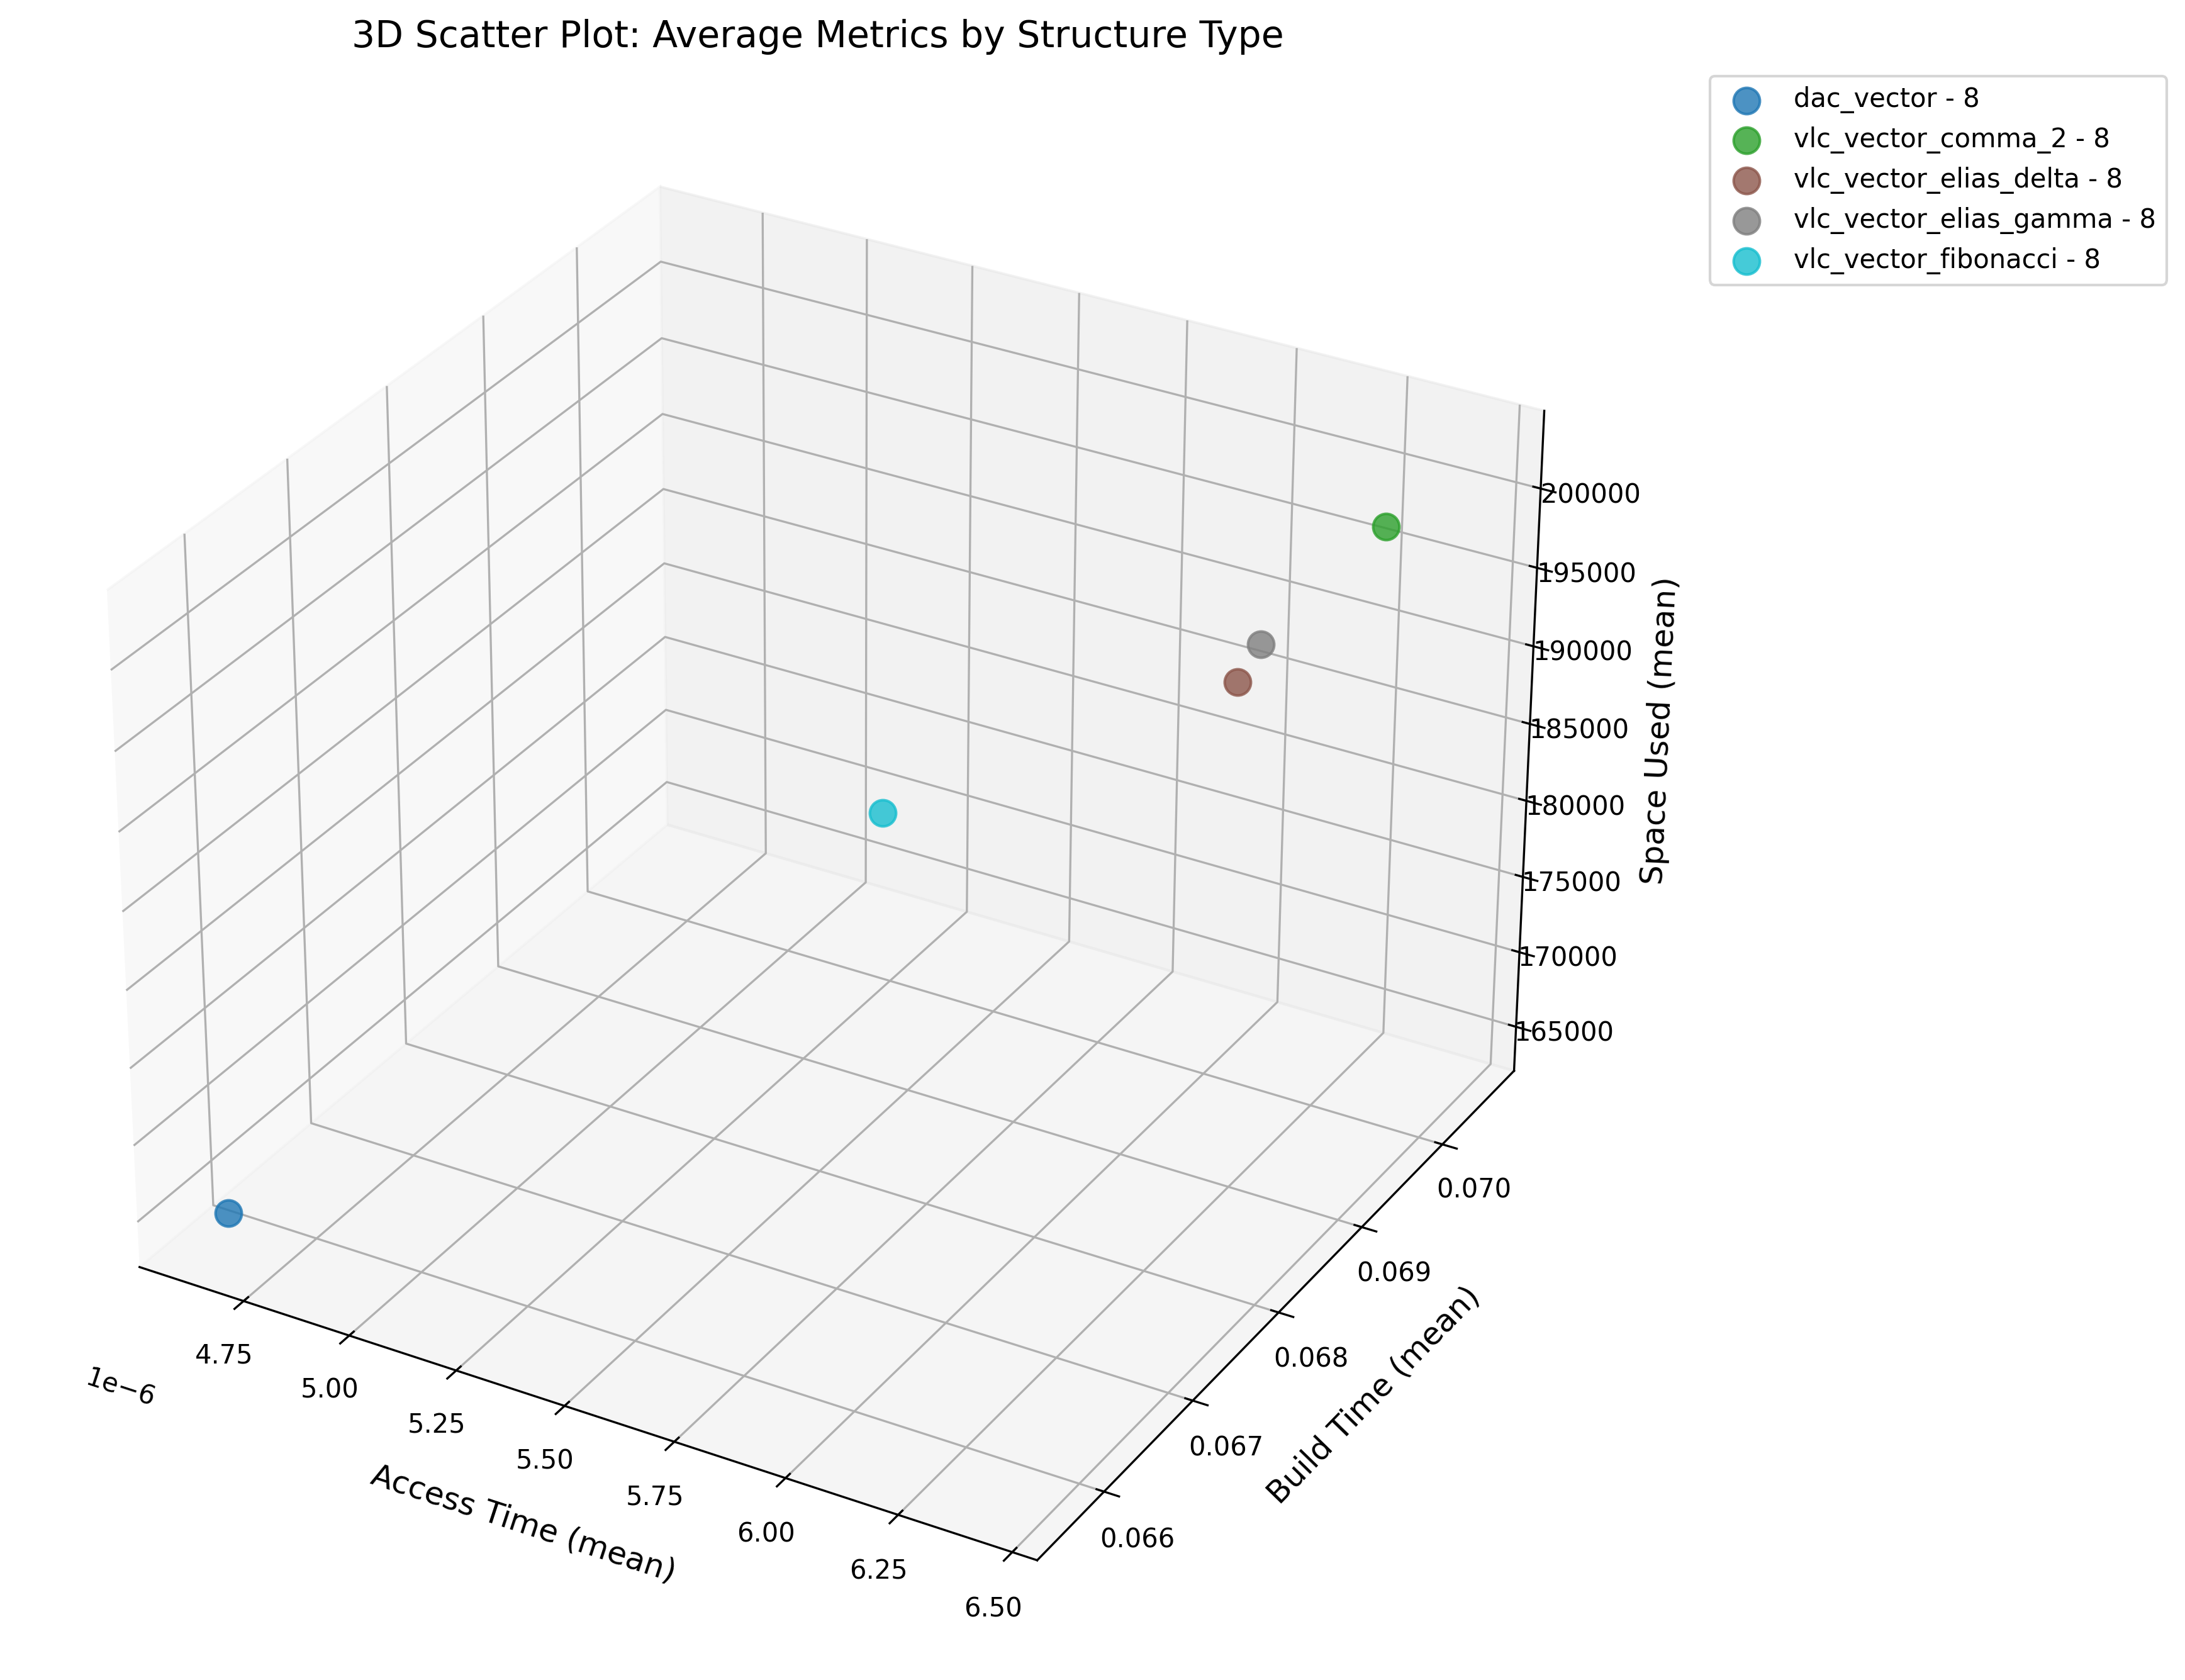
\includegraphics[width=0.8\textwidth]{alternatives/scatter_plot/3d_scatter_plot_structures.png}
\caption{Puntajes promedio de las estructuras de datos compactas}   
\label{fig:scatter_plot_structures}
\end{figure}

\begin{figure}[H]
\centering
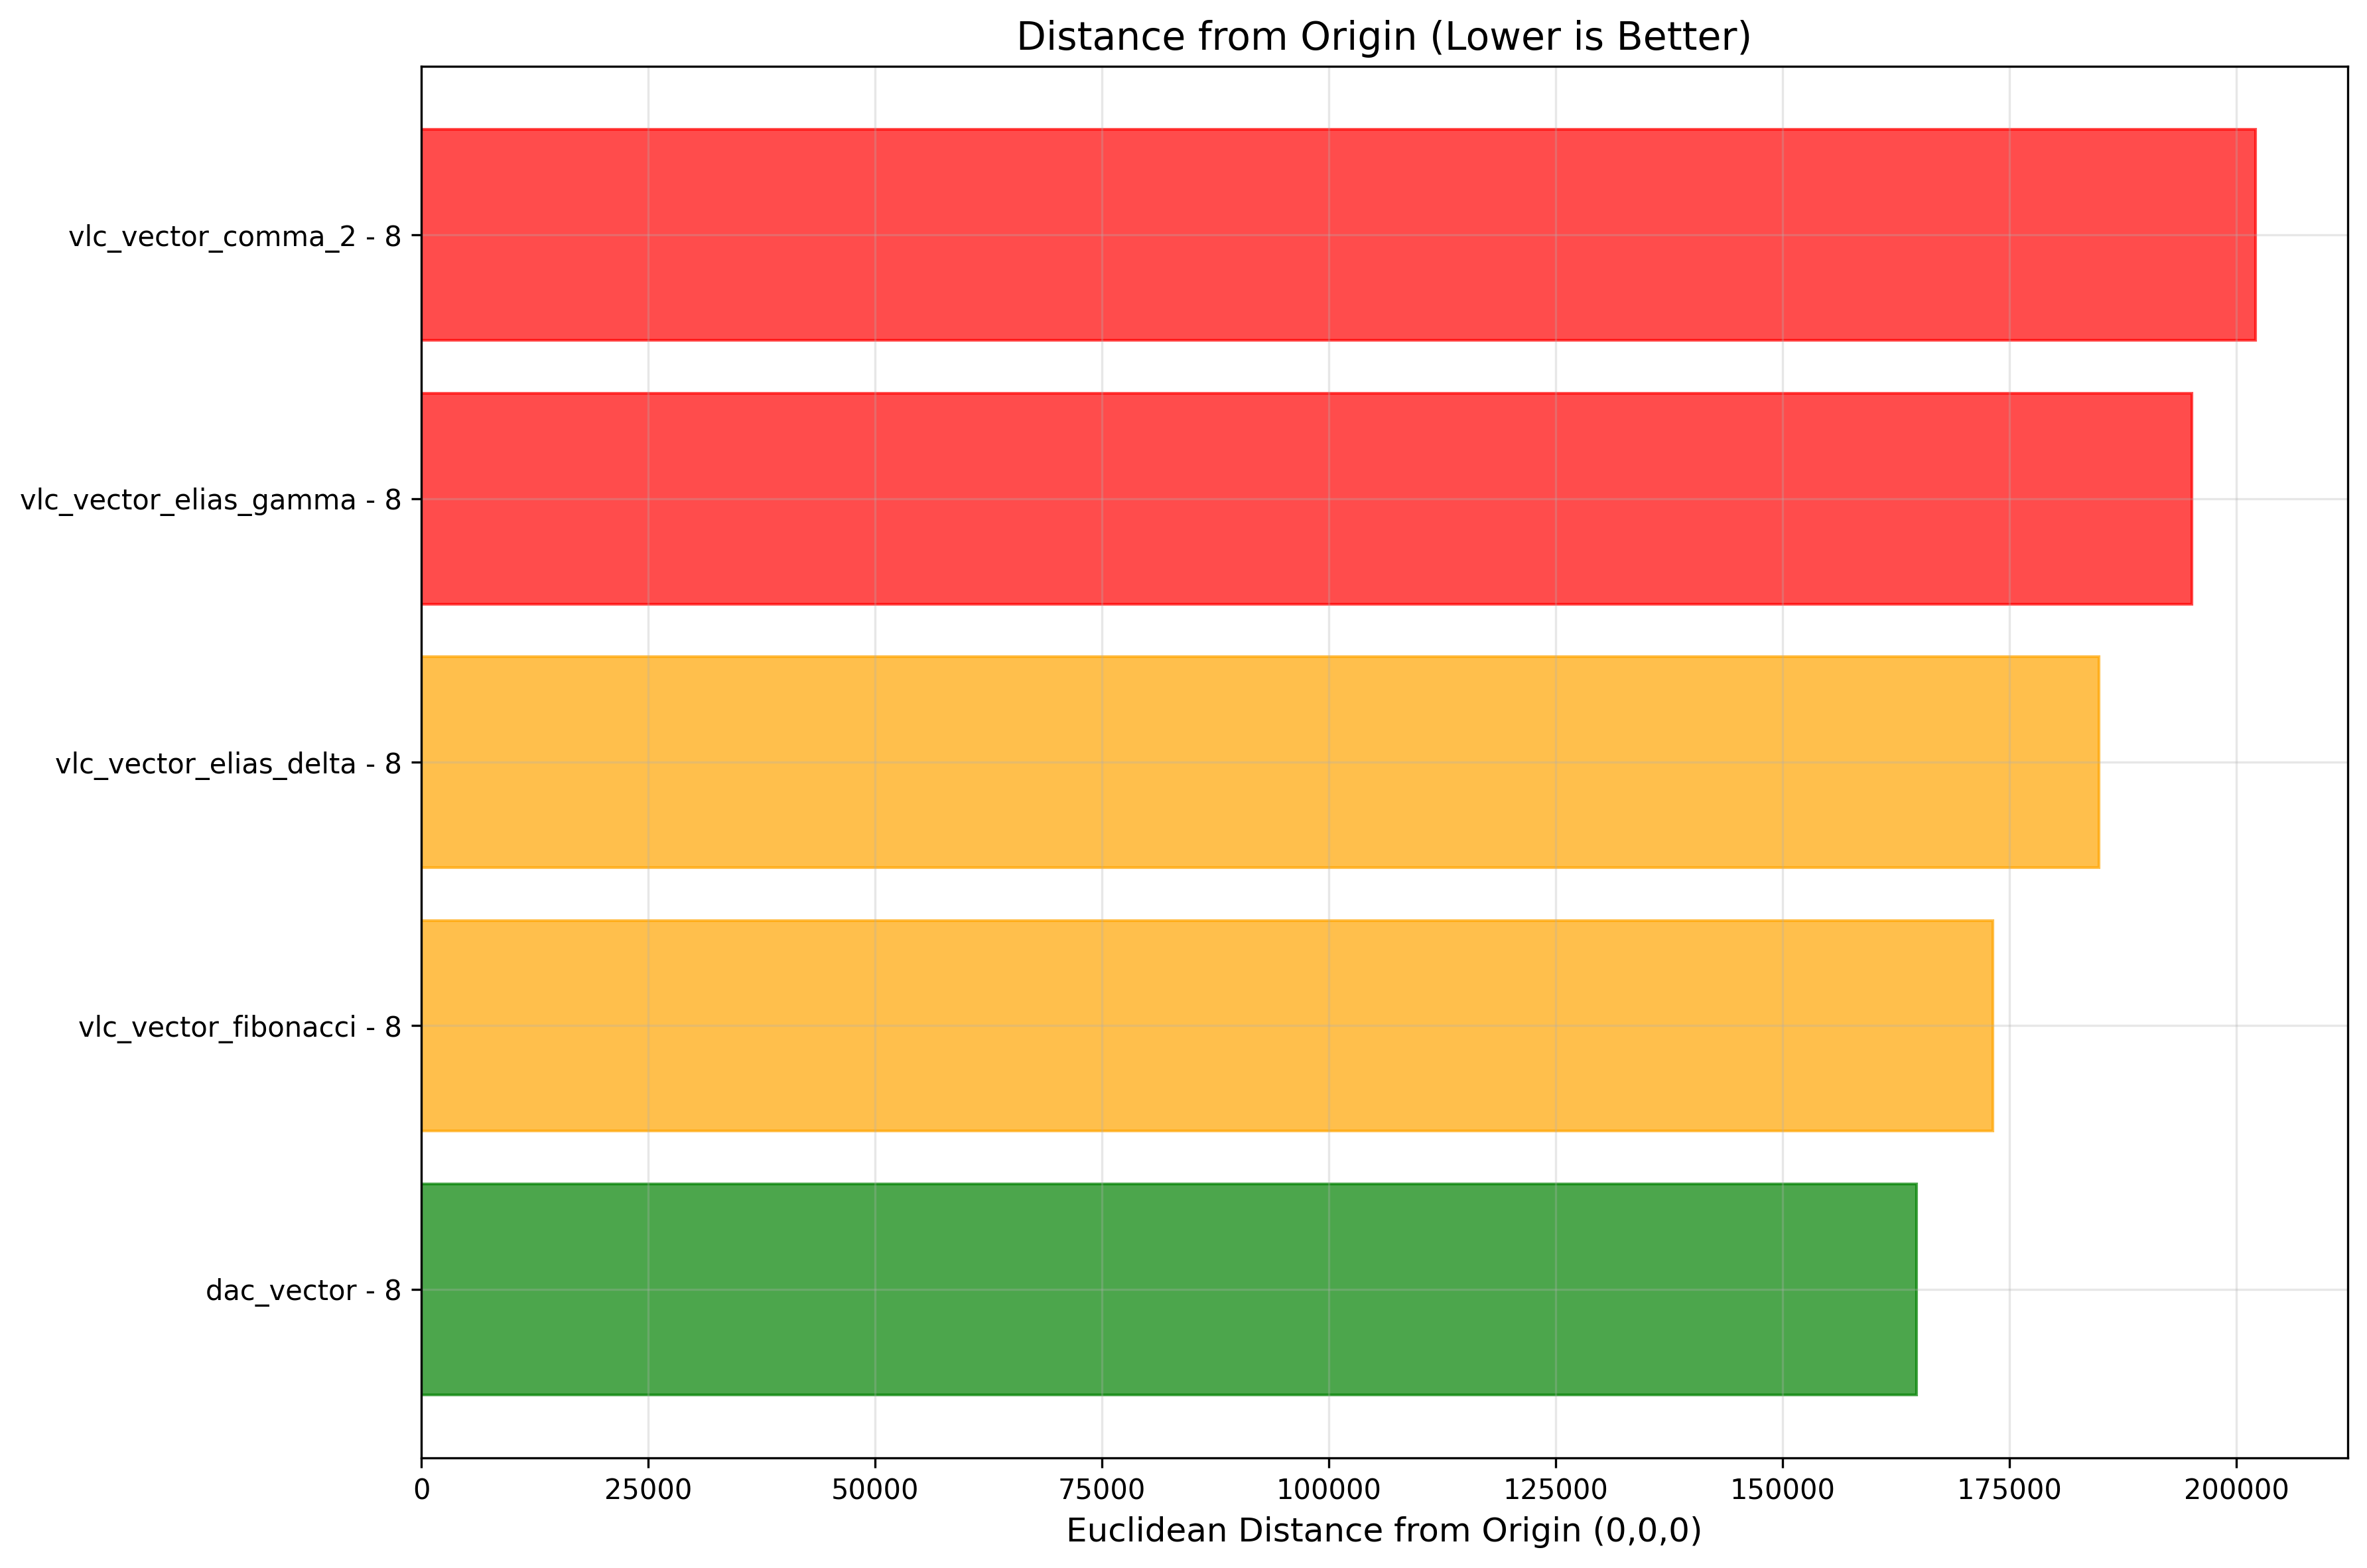
\includegraphics[width=0.8\textwidth]{alternatives/scatter_plot/euclidean_distance_from_ideal.png}
\caption{Distancia euclidiana promedio de las estructuras de datos compactas respecto al punto $(0, 0, 0)$}   
\label{fig:euclidian_distance_from_ideal}
\end{figure}

\begin{table}[h!]
\centering
\caption{Ranking of Structures by Access Time, Build Time, and Space Used}
\label{tab:structure_ranking}
\begin{tabular}{|c|l|r|r|r|}
\hline
\textbf{Rank} & \textbf{Structure} & \textbf{Access} & \textbf{Build} & \textbf{Space} \\
\hline
1 & dac\_vector - 8 & 0.000005 & 0.065626 & 164749.3 \\
\hline
2 & vlc\_vector\_fibonacci - 8 & 0.000005 & 0.070020 & 173138.0 \\
\hline
3 & vlc\_vector\_elias\_delta - 8 & 0.000006 & 0.070556 & 184829.3 \\
\hline
4 & vlc\_vector\_elias\_gamma - 8 & 0.000006 & 0.069361 & 195058.7 \\
\hline
5 & vlc\_vector\_comma\_2 - 8 & 0.000006 & 0.069731 & 202126.7 \\
\hline
\end{tabular}
\end{table}


A partir de la puntuación resultante, se seleccionan las estructuras de datos \textit{dac\_vector} y \textit{vlc\_vector\_fibonacci} como las más adecuadas para el sistema, ya que son las que obtuvieron los puntajes más favorables en la evaluación.